P.T.O.
\clearpage
\begin{figure}
  \caption{English Wikipedia, Page ID 4854639 (Ludvig Faddeev)}
  \centering

  \begin{subfigure}[b]{0.7\linewidth}
    \centering
    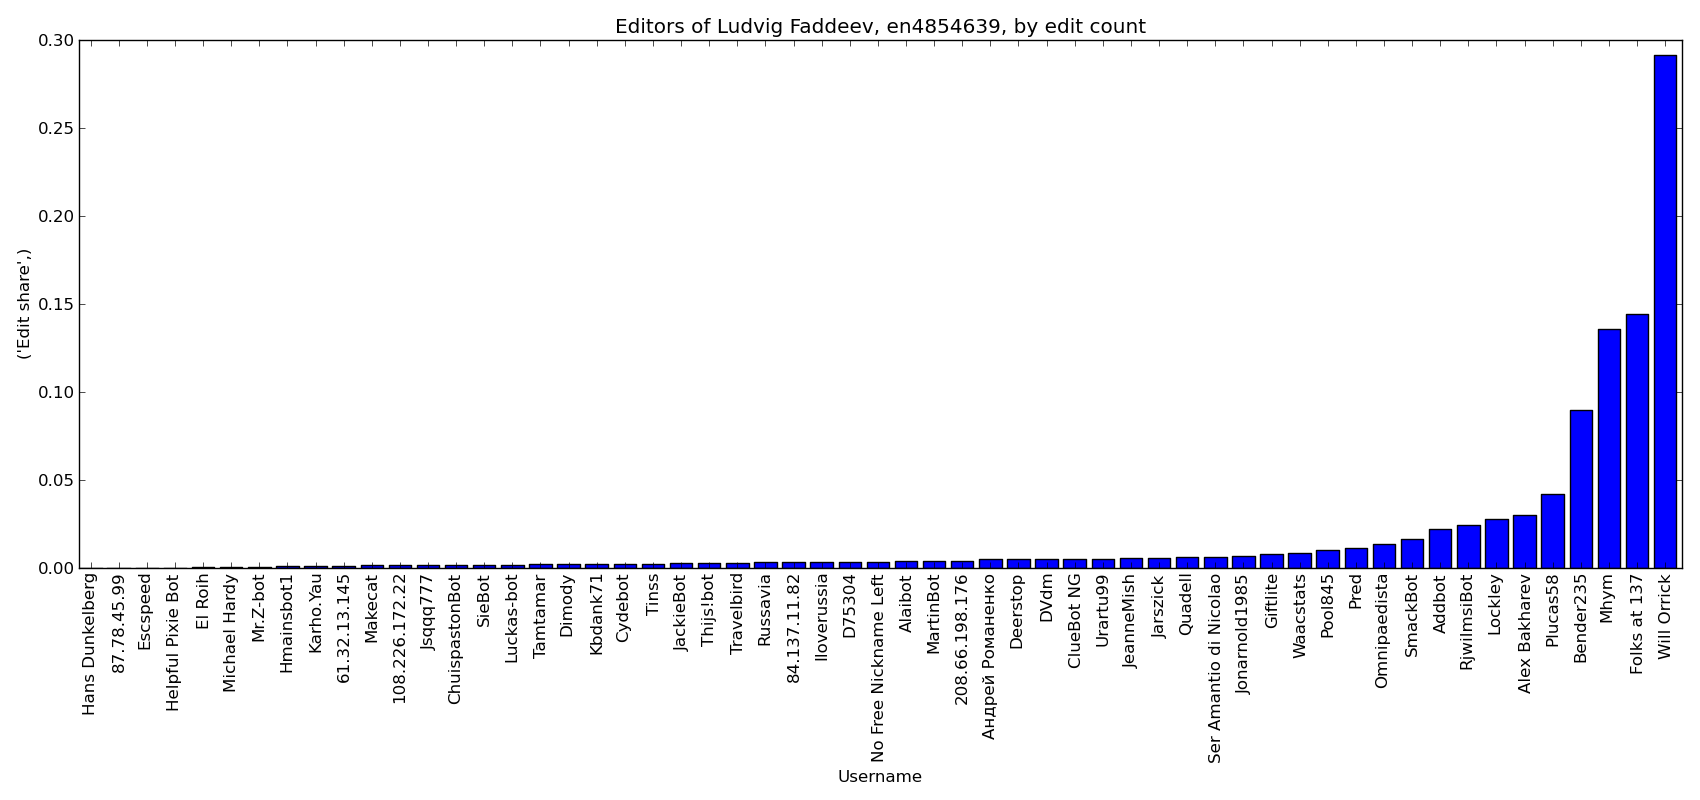
\includegraphics[width=\linewidth]{img/weightings/LudvigFaddeevUnweighted.png}
    \caption{Unweighted}
  \end{subfigure}
  \begin{subfigure}[b]{0.7\linewidth}
    \centering
    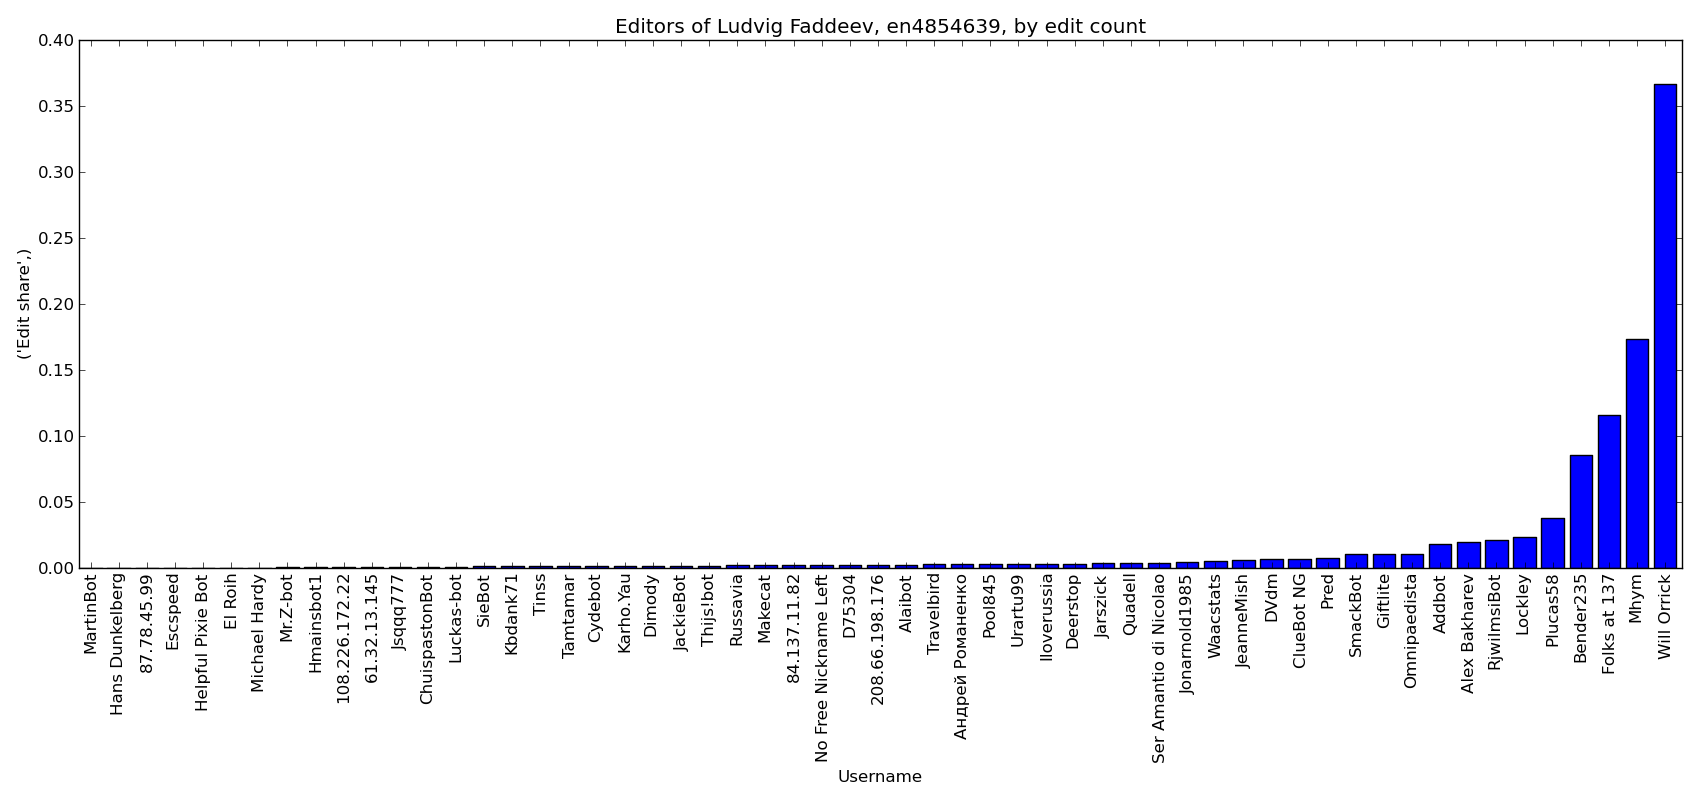
\includegraphics[width=\linewidth]{img/weightings/LudvigFaddeevUnweightedGradient.png}
    \caption{Unweighted with gradient}
  \end{subfigure}
  
  \centering
  \begin{subfigure}[b]{0.7\linewidth}
    \centering
    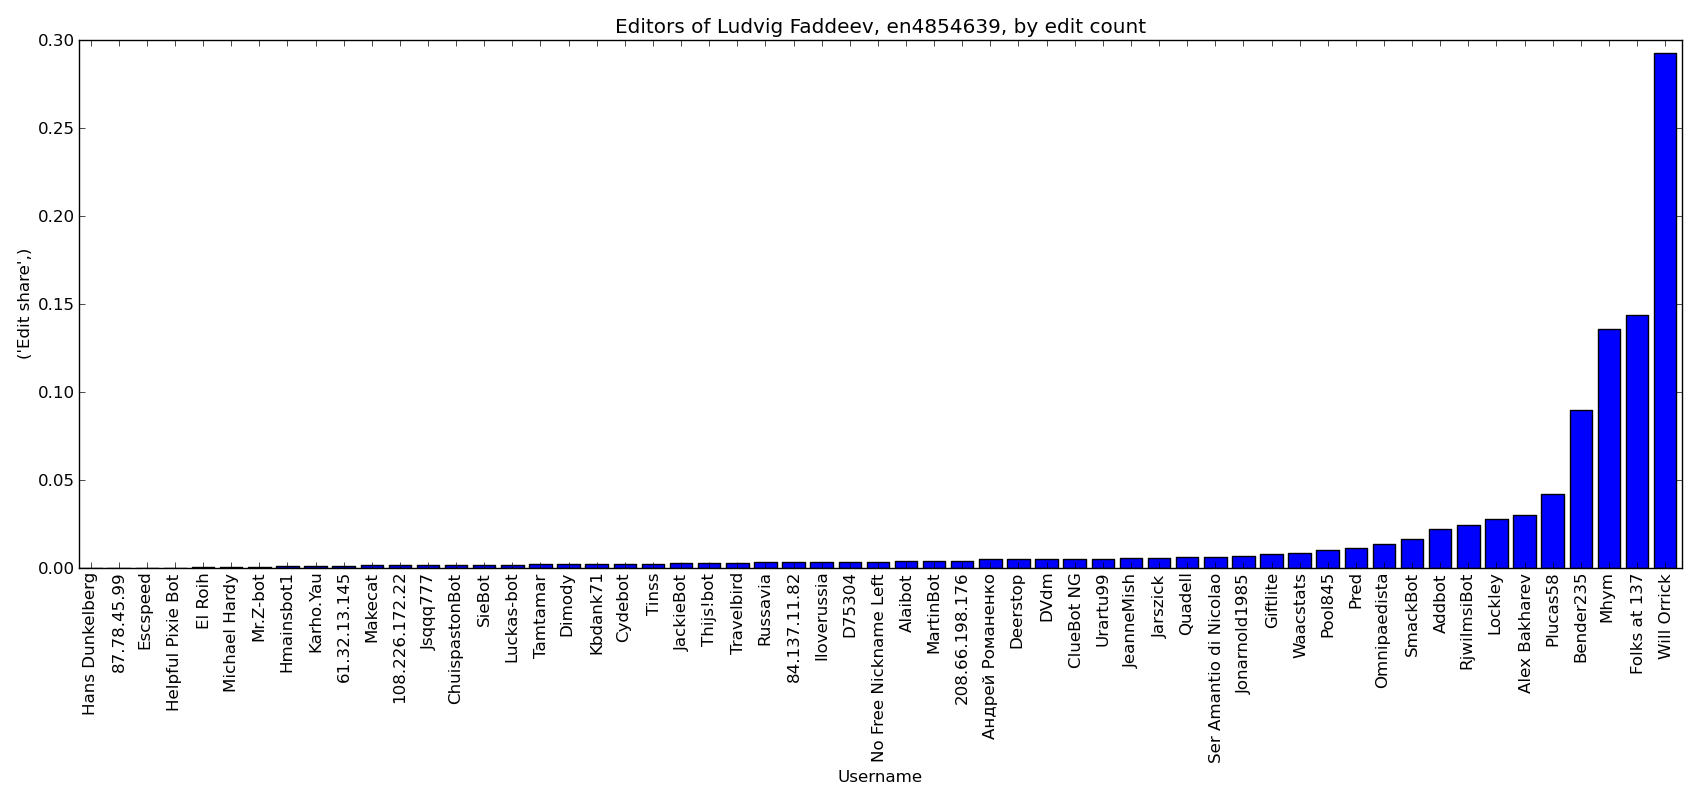
\includegraphics[width=\linewidth]{img/weightings/LudvigFaddeevStructure.png}
    \caption{...with double structure weight}
  \end{subfigure}
  \begin{subfigure}[b]{0.7\linewidth}
    \centering
    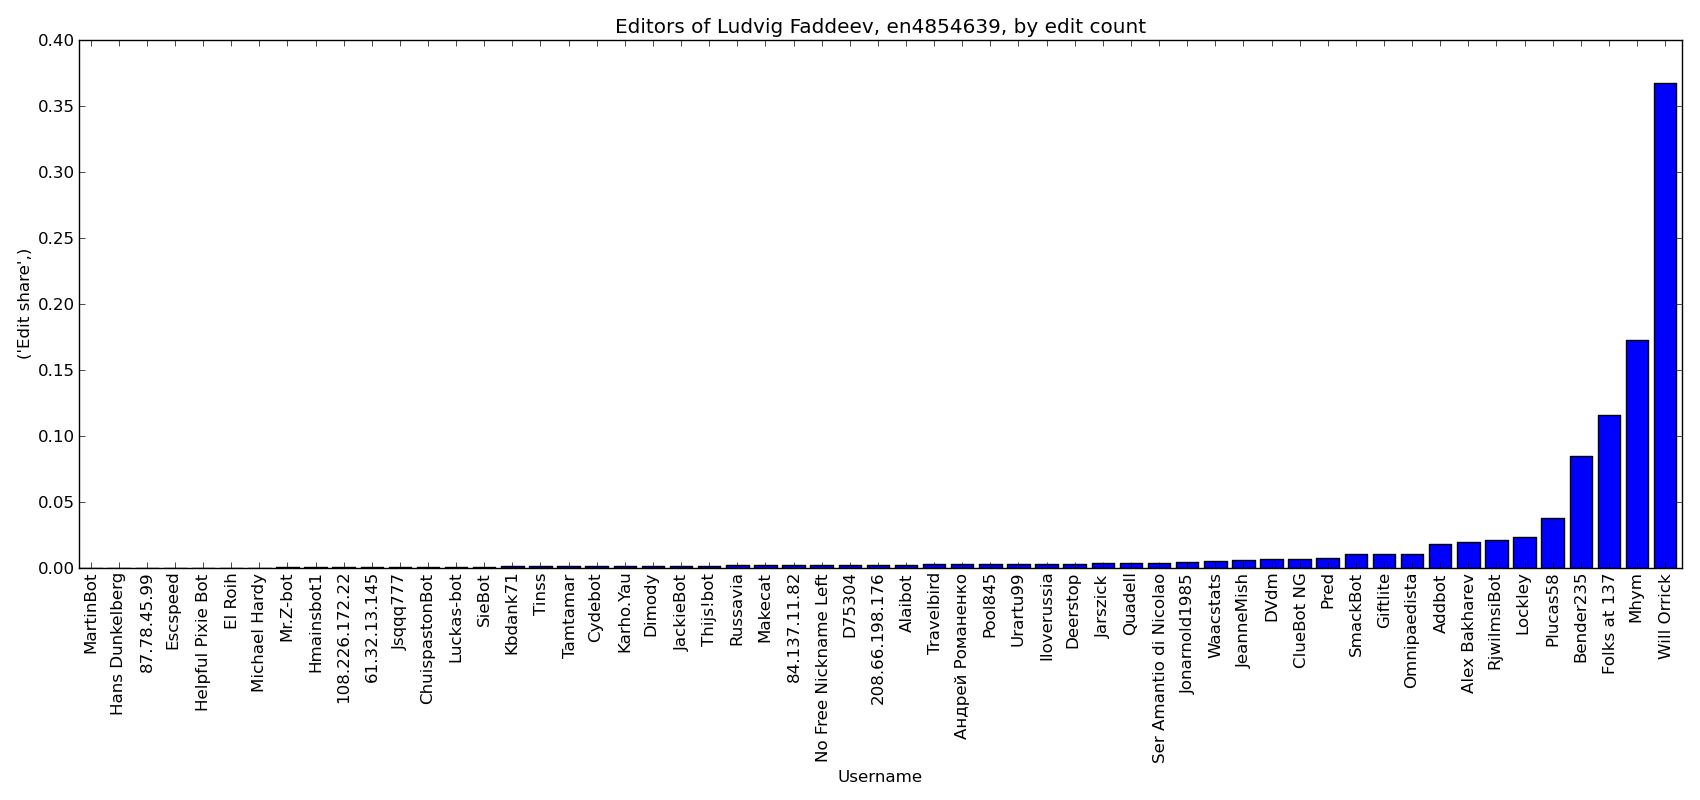
\includegraphics[width=\linewidth]{img/weightings/LudvigFaddeevStructureGradient.png}
    \caption{..plus gradient factor}
  \end{subfigure}
  
  
\end{figure}
\clearpage
\begin{figure}[H]
  \ContinuedFloat  
  \centering

  \begin{subfigure}[b]{0.7\linewidth}
    \centering
    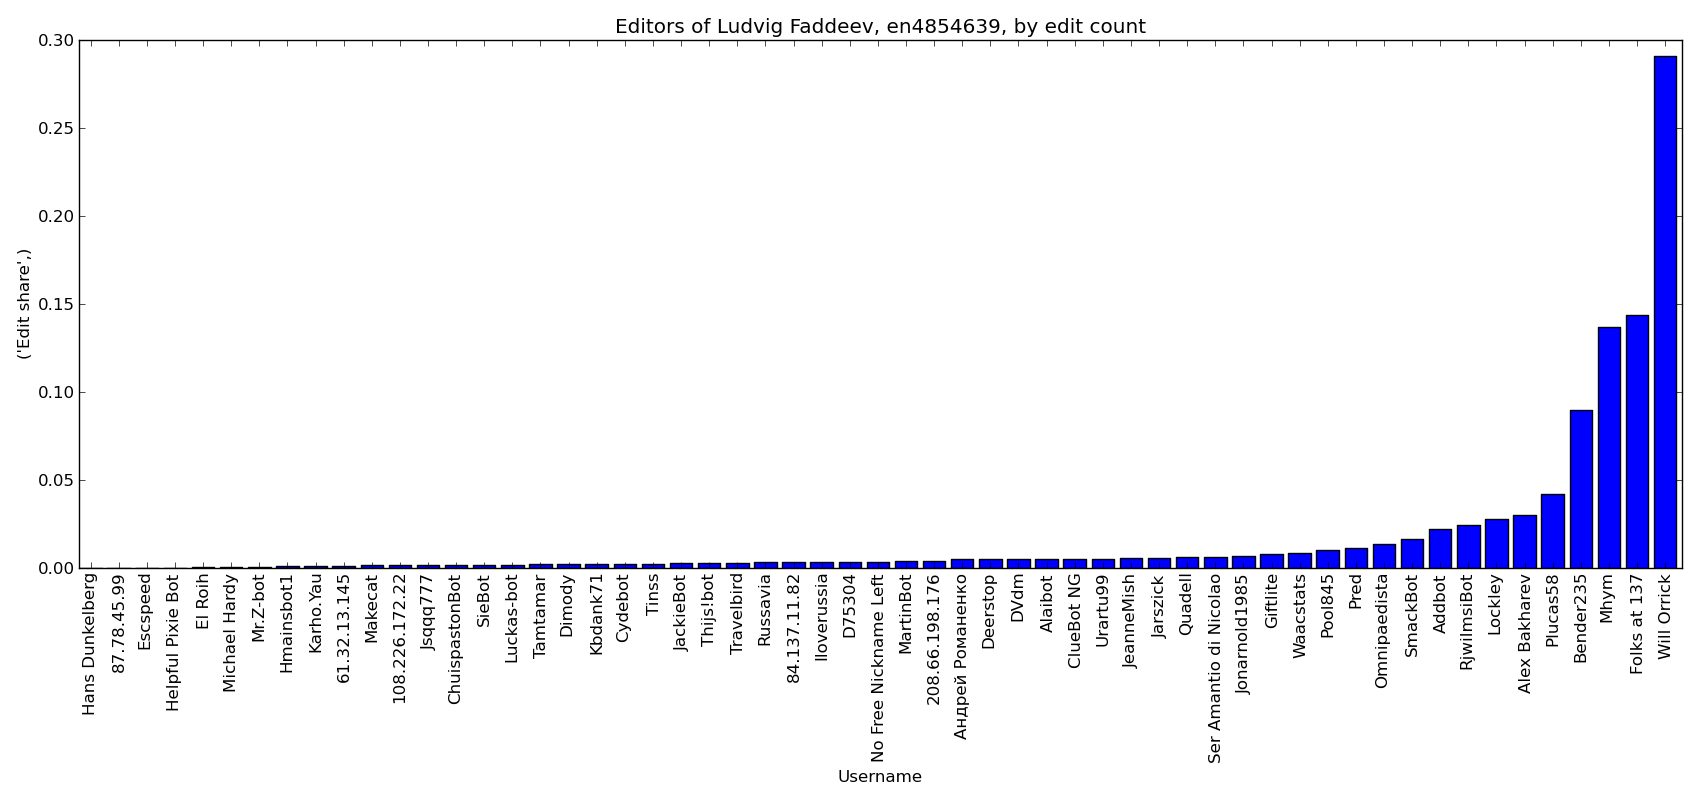
\includegraphics[width=\linewidth]{img/weightings/LudvigFaddeevMaths.png}
    \caption{...with double maths weight}
  \end{subfigure}


  \begin{subfigure}[b]{0.7\linewidth}
    \centering
    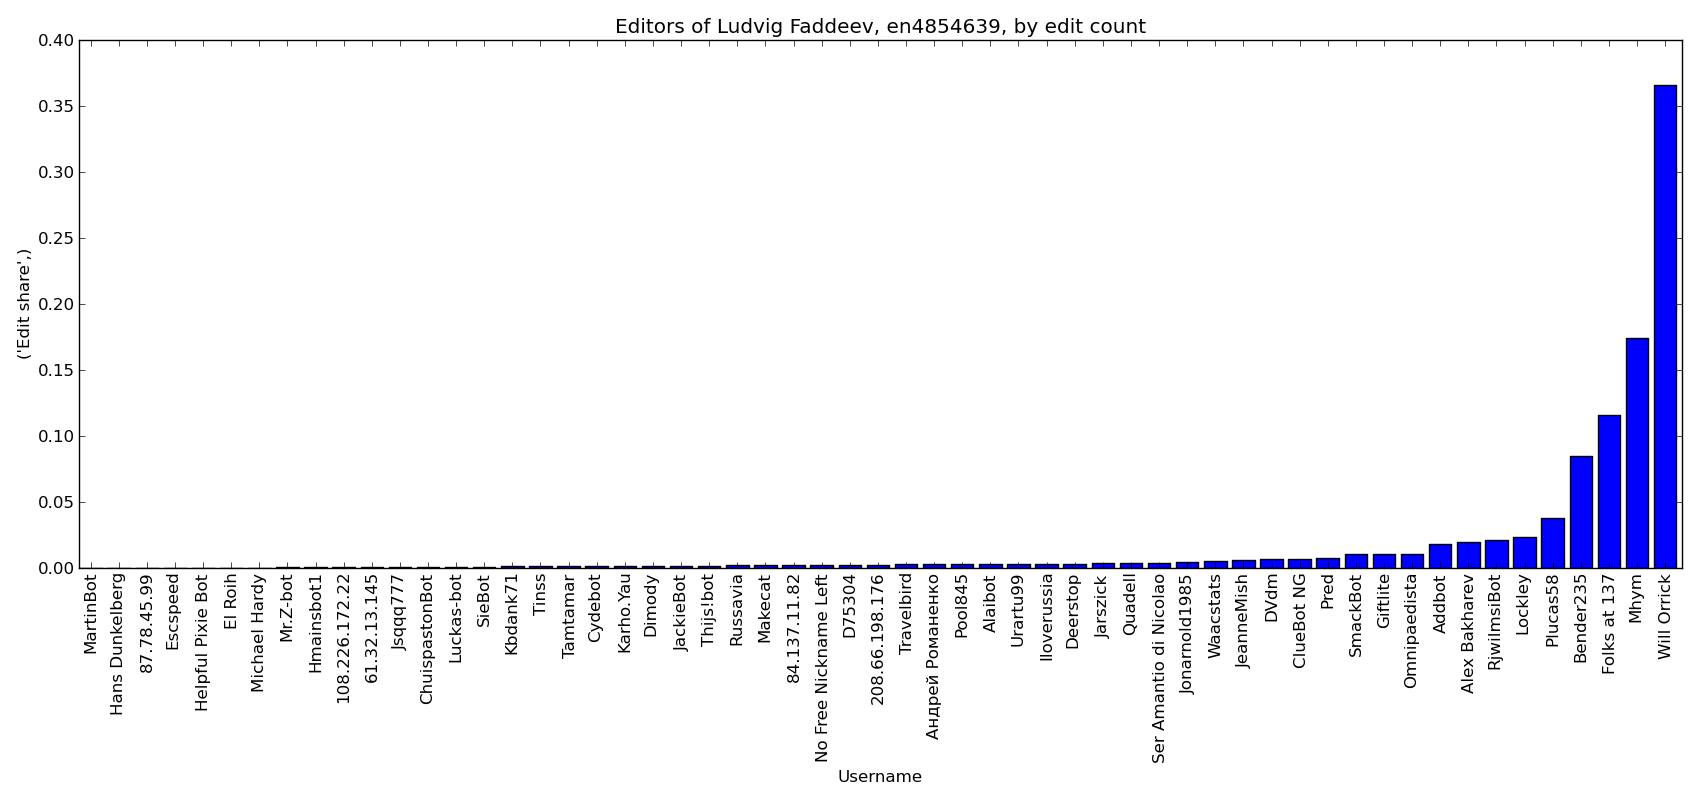
\includegraphics[width=\linewidth]{img/weightings/LudvigFaddeevMathsGradient.png}
    \caption{..plus gradient factor}
  \end{subfigure}
  

  \begin{subfigure}[b]{0.7\linewidth}
    \centering
    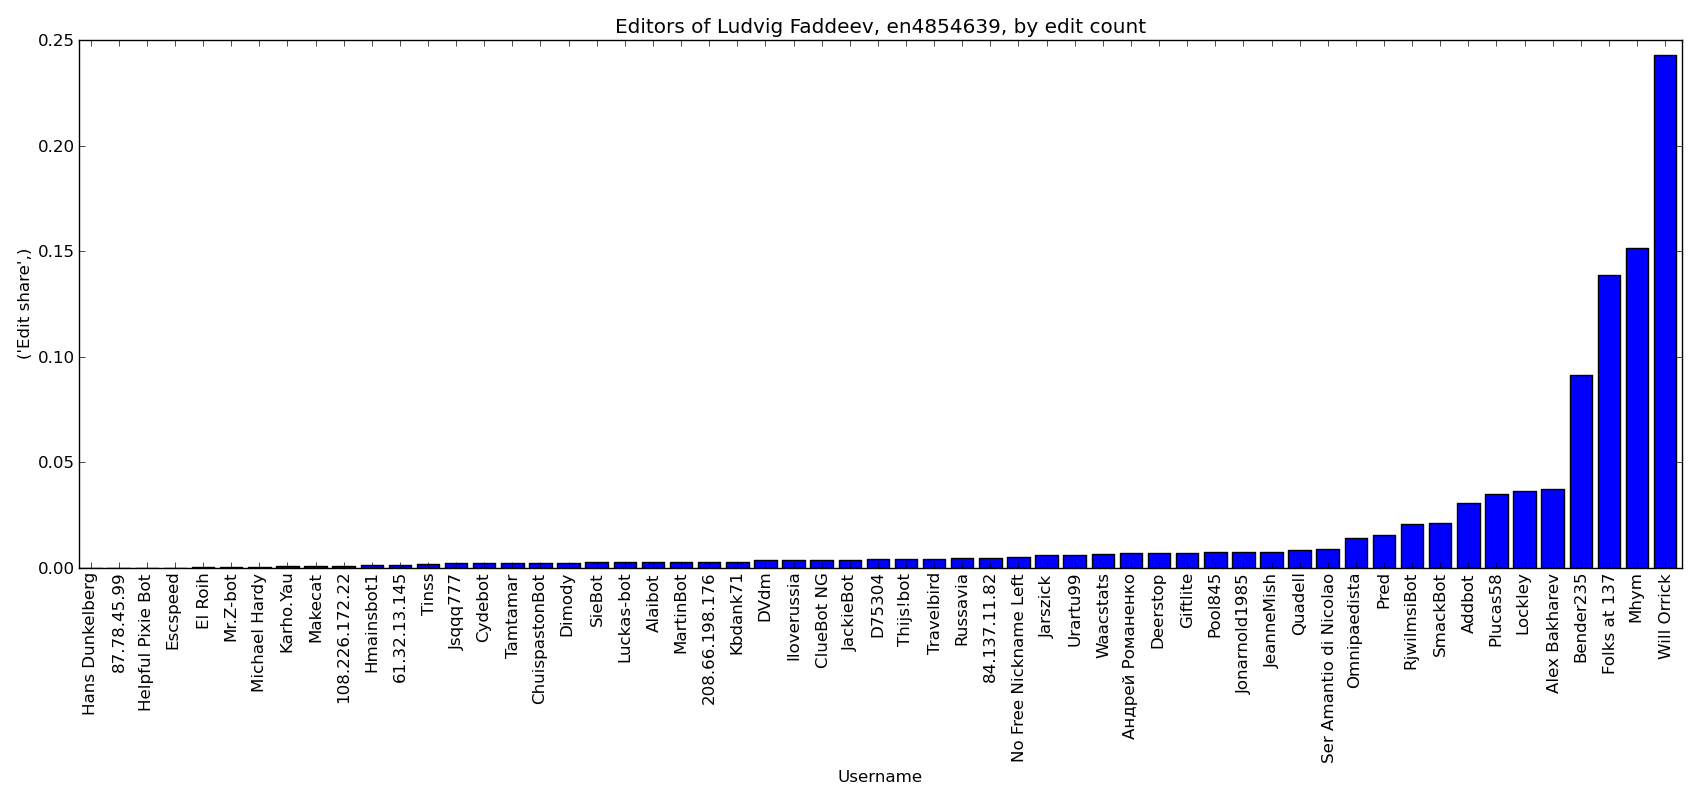
\includegraphics[width=\linewidth]{img/weightings/LudvigFaddeevLinks.png}
    \caption{...with double link weight}
  \end{subfigure}
  \begin{subfigure}[b]{0.7\linewidth}
    \centering
    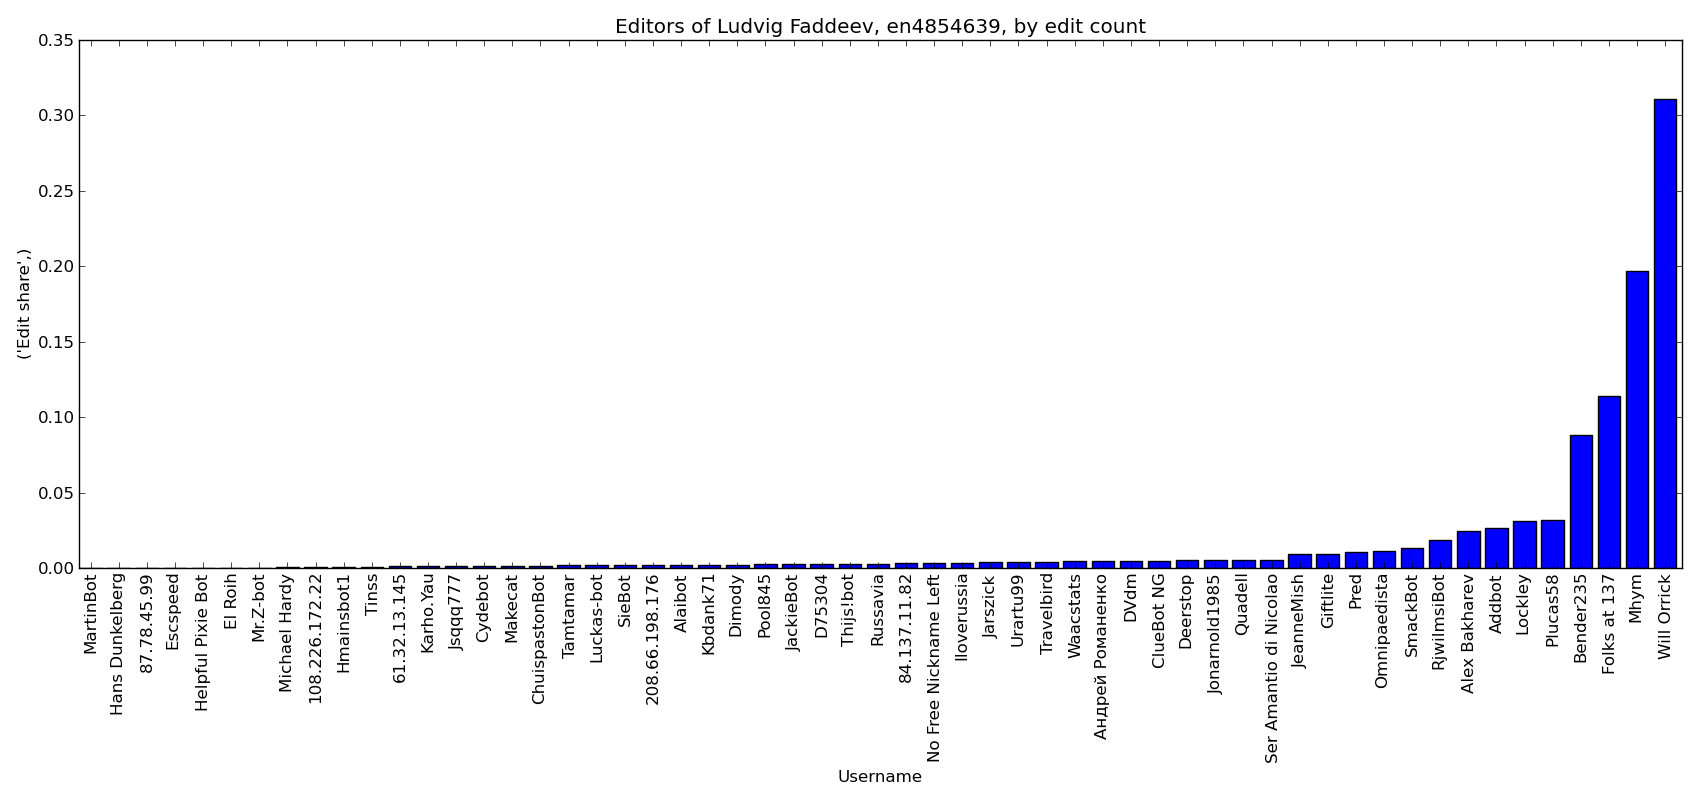
\includegraphics[width=\linewidth]{img/weightings/LudvigFaddeevLinksGradient.png}
    \caption{..plus gradient factor}
  \end{subfigure}
  
\end{figure}
\clearpage
\begin{figure}[H]
  \ContinuedFloat  
  
  \centering
  \begin{subfigure}[b]{0.7\linewidth}
    \centering
    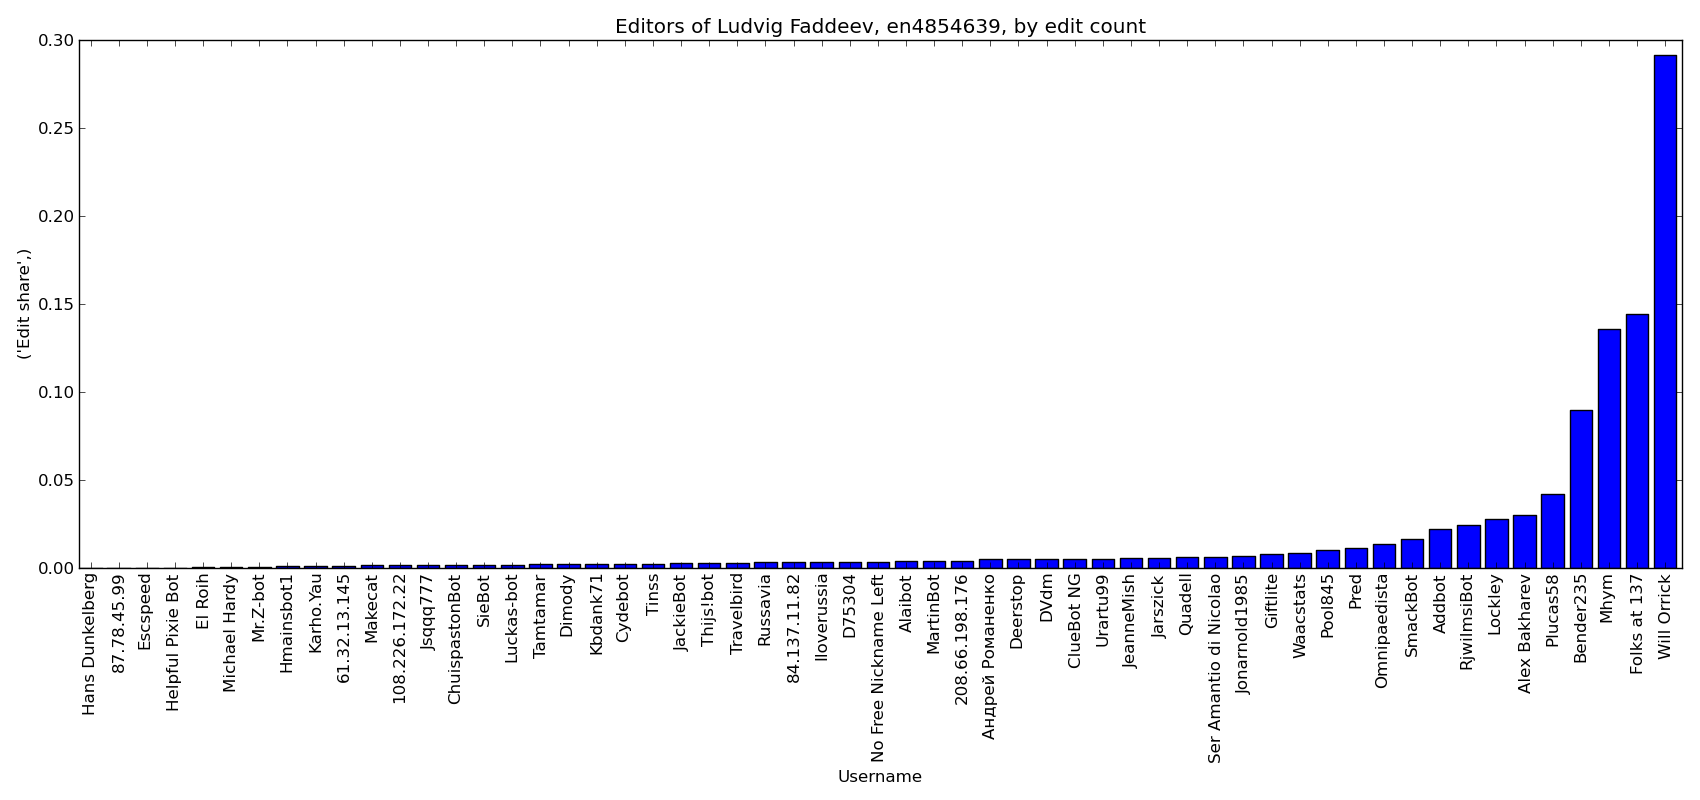
\includegraphics[width=\linewidth]{img/weightings/LudvigFaddeevfilesimages.png}
    \caption{...with double files / images weight}
  \end{subfigure}
  \begin{subfigure}[b]{0.7\linewidth}
    \centering
    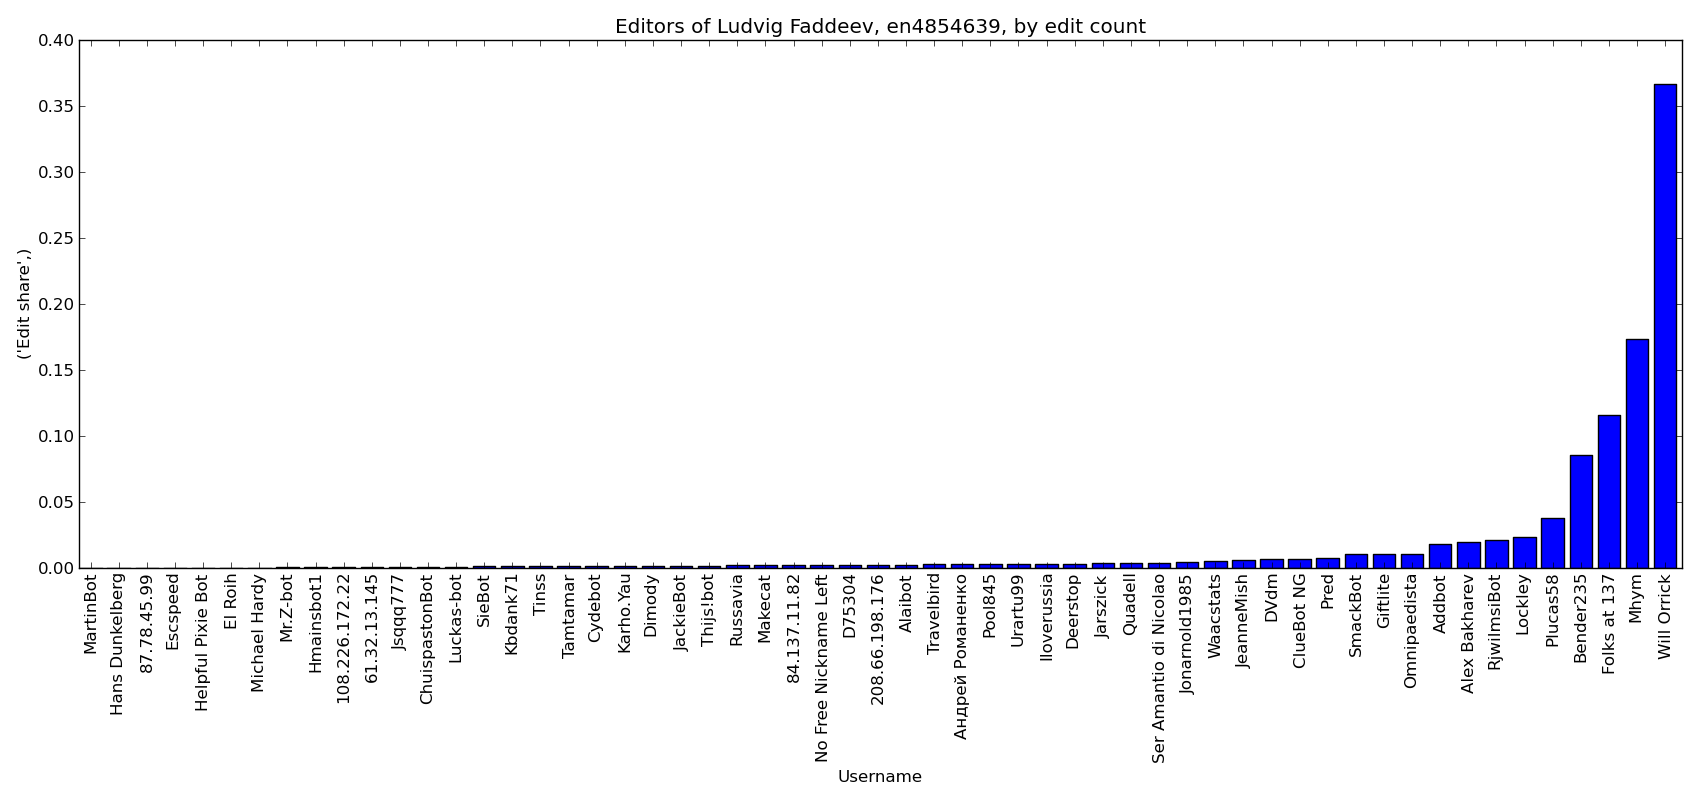
\includegraphics[width=\linewidth]{img/weightings/LudvigFaddeevfilesimagesGradient.png}
    \caption{..plus gradient factor}
  \end{subfigure}

  
  \begin{subfigure}[b]{0.7\linewidth}
    \centering
    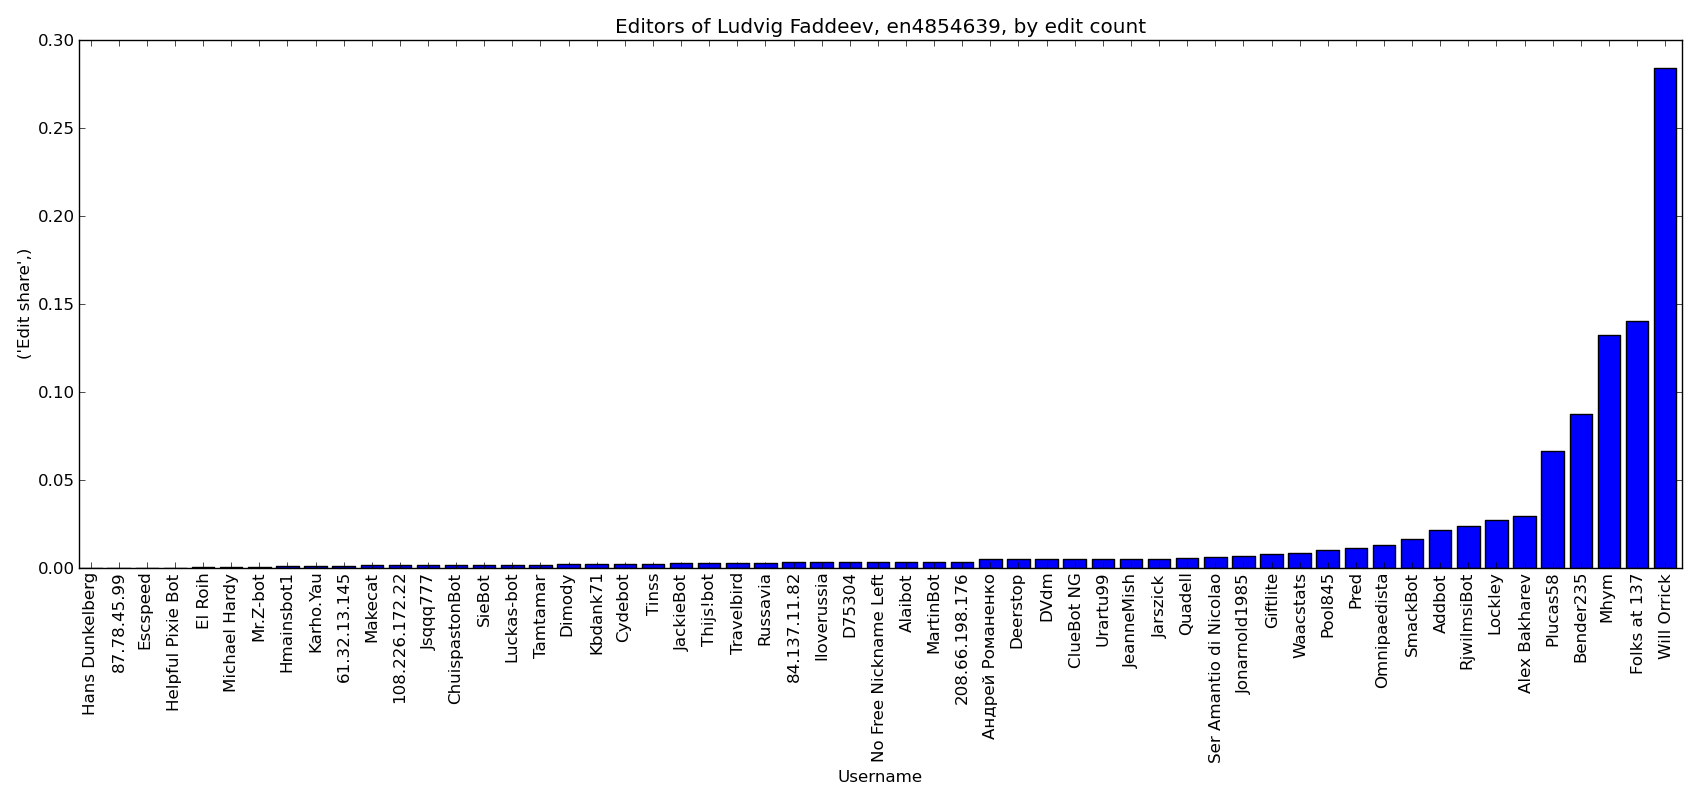
\includegraphics[width=\linewidth]{img/weightings/LudvigFaddeevCitations.png}
    \caption{...with double citations weight}
  \end{subfigure}
  \begin{subfigure}[b]{0.7\linewidth}
    \centering
    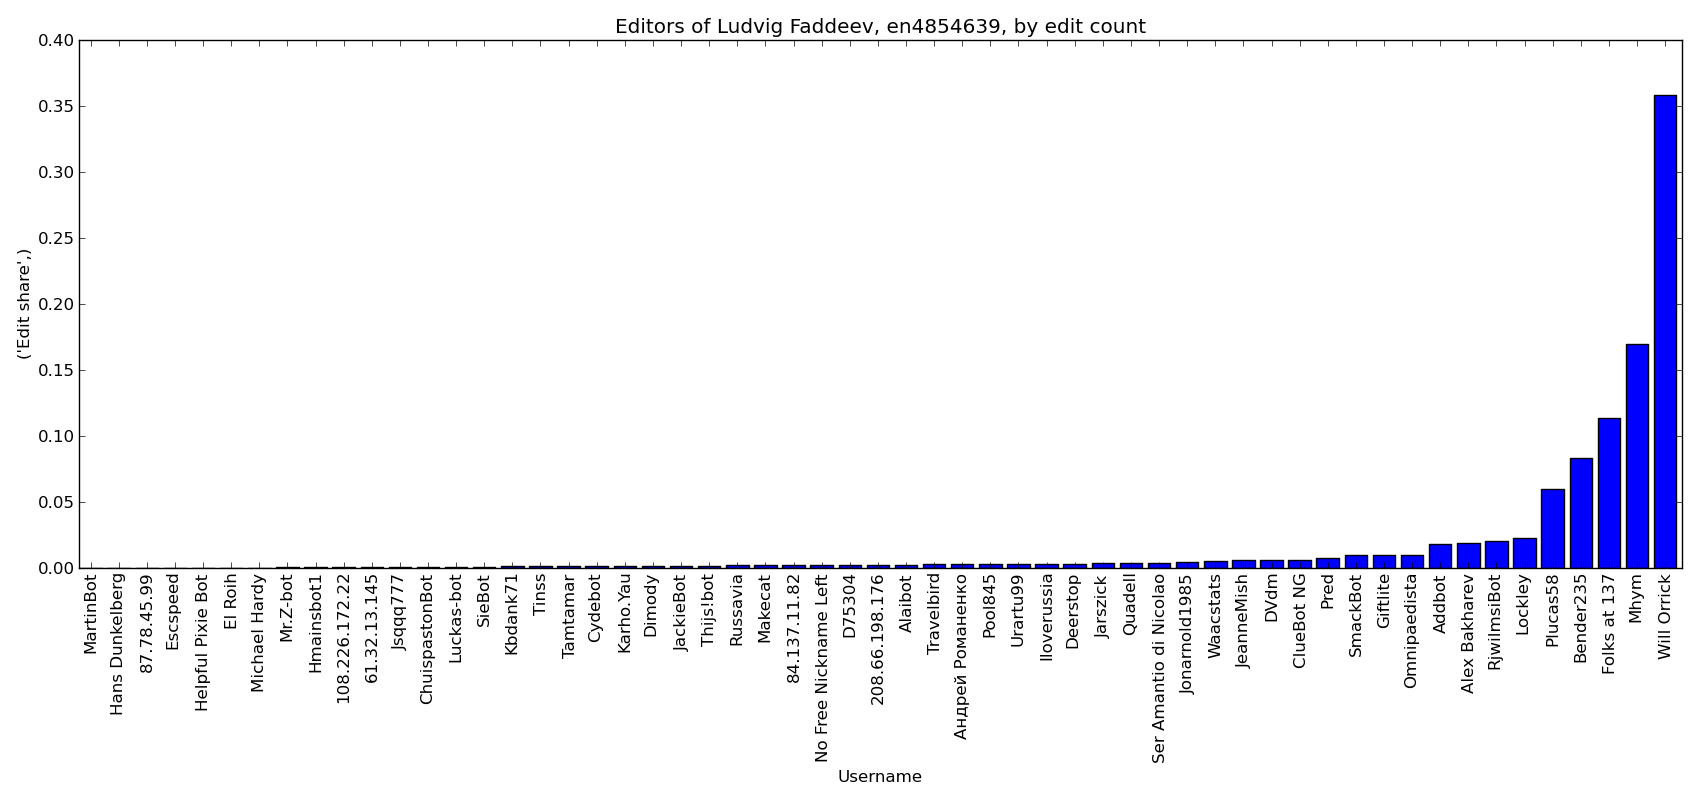
\includegraphics[width=\linewidth]{img/weightings/LudvigFaddeevCitationsGradient.png}
    \caption{..plus gradient factor}
  \end{subfigure}
  

\end{figure}
\clearpage
\begin{figure}[H]
  \ContinuedFloat  
  \centering
  \begin{subfigure}[b]{0.7\linewidth}
    \centering
    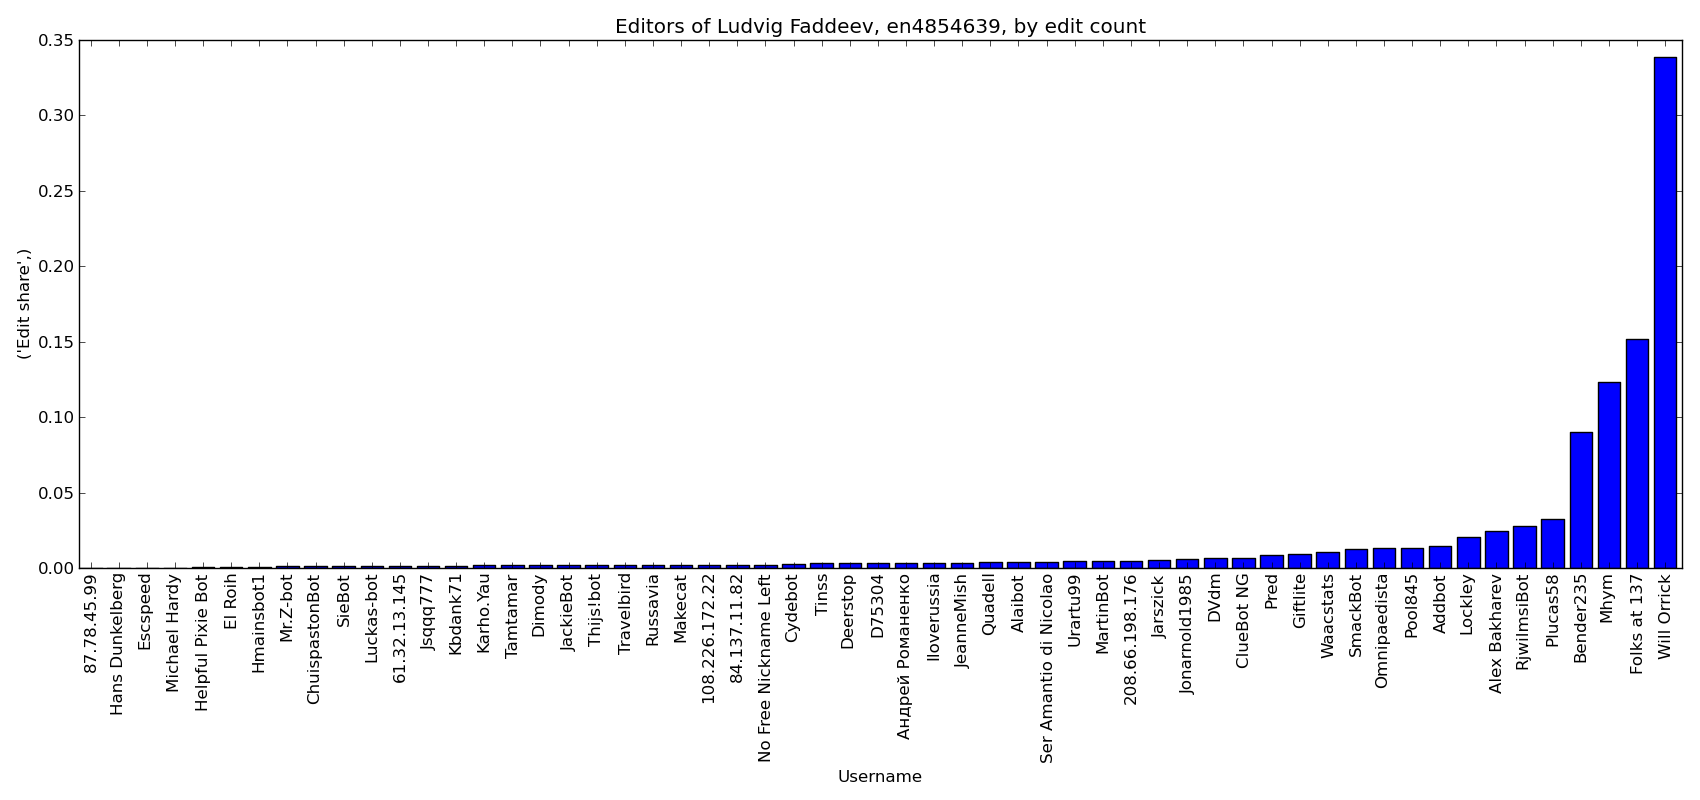
\includegraphics[width=\linewidth]{img/weightings/LudvigFaddeevNormal.png}
    \caption{...with double normal weight}
  \end{subfigure}
  \begin{subfigure}[b]{0.7\linewidth}
    \centering
    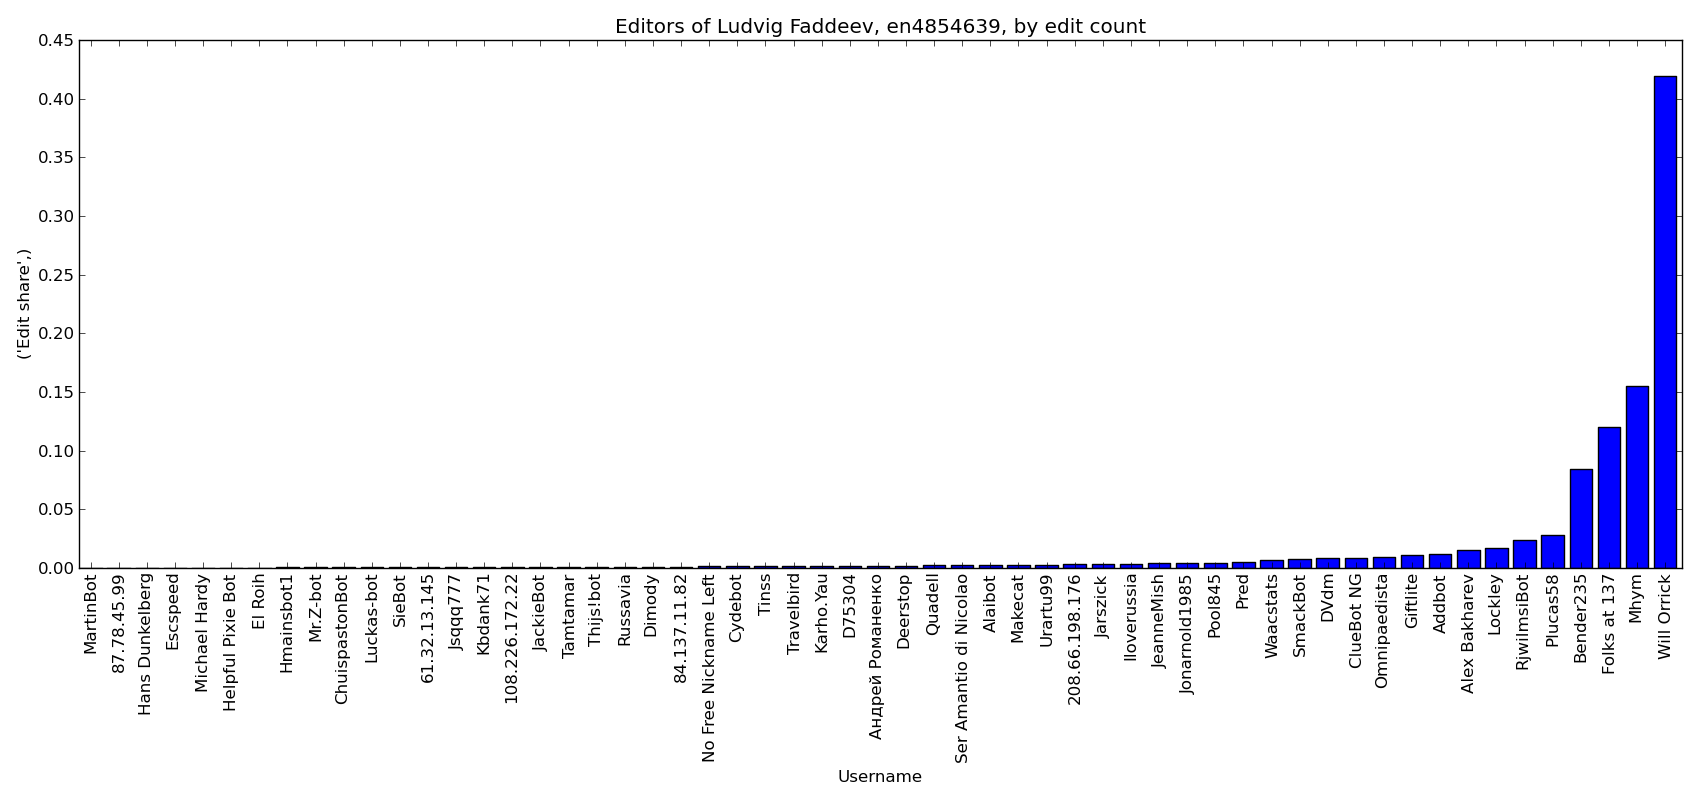
\includegraphics[width=\linewidth]{img/weightings/LudvigFaddeevNormalGradient.png}
    \caption{..plus gradient factor}
  \end{subfigure}
  

\end{figure}
